\documentclass[rmp, reprint, superscriptaddress, floatfix,amsmath]{revtex4-1}
\usepackage{longtable}
\usepackage{color}
\usepackage{graphicx}  % needed for figures
\usepackage[utf8x]{inputenc}
\usepackage{hyperref}
\usepackage{longtable}
\usepackage{xcolor}
\usepackage{soul}
\usepackage{multirow}
\usepackage{longtable}
\usepackage{xr-hyper}
\newcommand{\forcing}{\varepsilon}

\makeatletter
\newcommand*{\addFileDependency}[1]{% argument=file name and extension
  \typeout{(#1)}
  \@addtofilelist{#1}
  \IfFileExists{#1}{}{\typeout{No file #1.}}
}
\makeatother
 
\newcommand*{\myexternaldocument}[1]{%
    \externaldocument{#1}%
    \addFileDependency{#1.tex}%
    \addFileDependency{#1.aux}%
}
\myexternaldocument{main}

\definecolor{drab}{rgb}{0.59, 0.44, 0.09}
\newcommand{\Richard}[1]{{\color{drab}Richard: #1}}
\definecolor{celestialblue}{rgb}{0.29, 0.59, 0.82}
\newcommand{\Robert}[1]{{\color{celestialblue}Robert: #1}}
\definecolor{purple}{rgb}{0.459,0.109,0.538}
\definecolor{deepsaffron}{rgb}{1.0, 0.6, 0.2}
\newcommand{\Jan}[1]{{\color{deepsaffron}Jan: #1}}
\newcommand{\Emma}[1]{{\color{purple}Emma: #1}}
\definecolor{green}{rgb}{0.15, 0.6, 0.15}
\newcommand{\Valentin}[1]{{\color{green}Valentin: #1}}


\begin{document}

\title{Supplement: Impact of seasonal forcing on a potential SARS-CoV-2 pandemic}

\setcounter{figure}{0}
\renewcommand{\figurename}{Figure S}
\setcounter{table}{0}
\renewcommand{\tablename}{Table S}
\maketitle
The SIR model introduced in equations \ref{eq:SIR} describes the fraction of susceptible $S(t)$, exposed $E(t)$, and infected individuals $I(t)$ in a population. 
The fraction of recovered individuals $R$ is $R=1 - S - E - I$. 
An illustration of the model is presented in figure \ref{fig:schemeSIR}.

\begin{figure}[htb]
	\centering
	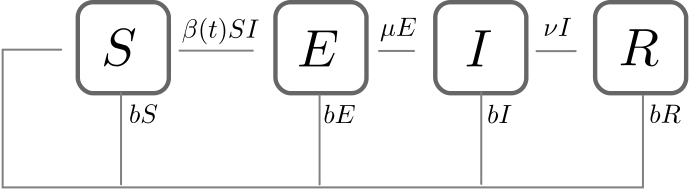
\includegraphics[width=0.9\columnwidth]{figures/SEIR_sketch.pdf}
	\caption{Illustration of the SEIR model used with its parameters.}\label{fig:schemeSIR}
\end{figure}



When simplifying the model even further and combining the categories of exposed and infectious into one class of infected individuals, the model can be solved analytically.
The simplified system has a steady state
\begin{equation}
\begin{split}
S_0 &= \frac{\nu + b}{\beta} = \frac{1}{R_0} \\
I_0 & = \frac{b(R_0-1)}{\beta}
\end{split}
\label{eq:fixed_point}
\end{equation}
where $\nu$ now is the inverse of average time from exposure to recovery.
This steady state exists when the parameter $R_0 > 1$. For cases where $R_0 < 1$ the epidemic dies out as each infected person generate less than one subsequent infection. 

For our analysis of seasonal CoVs, it is instructive to study the stability of this steady state of the simplified SIR (not SEIR) model. 
It is easy to show that the quantities $[S,I]$ tend to show damped oscillations around the fixed points in Eq.~\ref{eq:fixed_point} with a period
\begin{equation}
T = \frac{4\pi}{\sqrt{4b(\nu(R_0-1) - b) - R_0^2b^2}}
\label{eq:period}
\end{equation}
This behavior is intrinsic to the system and holds whenever transmissibility is constant.

SIR models can show resonance phenomena when the period is about one or two years \citep{dushoff_dynamical_2004,chen_regular_2017}.
Resonance is less likely when the period is much longer than the the period of annual forcing.
Fig.~\ref{fig:intrinsicPeriod} shows the intrinsic period for the parameter range considered and two durations of immunity (left: 10 years, right: 5 years). 
Our parameters choices for $\nu$ $\beta$ lie in the center of the graphs in Fig.~\ref{fig:intrinsicPeriod}. 
For $b=0.1/y$, we expect an intrinsic period is around 3 years, suggesting that resonance is unlikely and if it occurs would lock into 3 year patters.
For $b=0.2/y$, the intrinsic period is closer to 2 years and biennial resonance is possible. 
The data, however, don't suggest strong biennial patterns such that we don't think resonance is a major contributor to seasonality.

Similarly, in the simplified SIR (not SEIR) model, the initial growth of the number of cases can be expressed analytically.
In a fully susceptible population, the number of infected individuals initially grows as $I(t)\sim e^{(\beta-\nu-b)t} = e^{(R_0-1)t/(\nu+b)}$.
The doubling time is $\tau_2 = (\nu+b)\log(2)/(R_0-1)$.
Since $b\ll \nu$, we can safely neglect $b$ in the early phase of the pandemic, but it is important when interpreting endemic seasonal CoV data. 
For detailed discussion of the effect of generation times and incubation periods on the initial exponential growth, see \citep{wallinga_how_2007}.


\begin{figure*}[htb]
	\centering
	\includegraphics[width=0.9\columnwidth]{figures/Period_phase_space_b_0.1.pdf}
	\includegraphics[width=0.9\columnwidth]{figures/Period_phase_space_b_0.2.pdf}
\caption{Length of the intrinsic period of the SIR model for $\beta$ and $\nu$ values in the range explored in this paper. The duration of immunity is assumed to be $10$ years in the panel on the left and 5 years in the panel on the right. The dark blue region corresponds to $R_0<1$. }
	\label{fig:intrinsicPeriod}
\end{figure*}


\subsection*{Migration between subpopulations}

In the model for seasonal CoVs, we account for the exchange of CoVs with the rest of the world through an additional transition of susceptibles to the exposed category with a rate that is the product of a migation rate and the probability of being exposed abroad. 
Beyond that, no additions to Eq.~\ref{eq:SIR} are necessary.

For the multipopulation models of SARS-CoV-2 pandemics, we model migration as loss terms to each category with a population specific migration rate, followed by redistributions of the pooled migrants to random population according the population specific migration rate. 
Such migration is operating in Figures \ref{fig:nCov_predictions}, \ref{fig:global_3_panel} and \ref{fig:endemic}. 

\subsection*{Effect of infection control measures}
The SIR model as formulated in Eq.~\ref{eq:SIR} accounts for seasonality but otherwise assumes the transmission dynamics is constant. 
In reality, individuals change their behavior when they are aware of a contagious disease.
This in particularly true for the current SARS-CoV-2 outbreak where tens of millions of people are under quarantine measures and travel restrictions.
In order to account for such behavioral changes, we add a factor $H$ to equation \ref{eq:SIR} that modulates transmission:
\begin{equation}
\frac{d}{dt} I =  -(\nu+b) I + (1-H)\beta S I + i
\end{equation}
where $H = c\cdot\frac{I^3}{(K^3+I^3)}$ with $c$ the value of the containment parameter. 
The term $H$ is a Hill function of order 3 and inflection point $K$. 
We use this to model a decrease in the rate of new infection smoothly decrease by a factor $c$. 
We used $c=0.5$ and $K=0.03$, implying that once a disease is at a prevalence of 3\%, containment measures reduce transmission by 50\%.
The effect of prevention and control is difficult to assess at present and will certainly vary in time and space. 

\bibliography{bib}
\begin{figure}
    \centering
    \includegraphics[width=0.5\textwidth]{figures/fraction_positive_HKU1_OC43.pdf}
    \caption{Seasonal variation of HKU1/OC43 CoV positive tests in Stockholm, Sweden. }
    \label{fig:seasonal_variation_supp}
\end{figure}

\begin{figure*}[h]
	\centering
	\includegraphics[width=0.9\textwidth]{figures/scenario_subplot_0.5.pdf}
	\caption{{\bf Model predictions for SARS-CoV-2 case numbers in temperate zones for a pandemic scenario, with varying $\langle R_0\rangle$ and migration.} This is the same plot as shown on the left of Figure \ref{fig:nCov_predictions} with $\forcing=0.5$, however here $\langle R_0\rangle$ varies from 1.3 - 3 and Migration varies from 0.1\% to 10\% per year. Higher migration rates (towards the bottom of the figure) result in earlier introductions and higher likelihood of a peak in early 2020.
	The scenarios with low $\langle R_0\rangle$ are clearly counter-factual. 
	Similarly, higher $\langle R_0\rangle$ (towards the right of the figure) results in more rapid growth and a higher likelihood of an early peak.}
	\label{fig:scenarios_supp}
\end{figure*}


\begin{figure*}[h]
	\centering
	\includegraphics[width=0.9\textwidth]{figures/scenario_subplot_0.15.pdf}
	\caption{{\bf Model predictions for SARS-CoV-2 case numbers in temperate zones for a pandemic scenario, with varying $R_0$ and migration.} This is the same plot as shown on the left of Figure \ref{fig:scenarios_supp} but with $\forcing=0.15$. All scenarios result in a single peak.}
	\label{fig:scenarios_weak_supp}
\end{figure*}


\begin{figure*}[h]
	\centering
	\includegraphics[width=0.9\columnwidth]{{figures/peak_ratio_0.3}.pdf}
	\includegraphics[width=0.9\columnwidth]{{figures/peak_ratio_0.7}.pdf}
	\caption{{\bf Ratio of first and second peak in temperate zone pandemic scenarios, with varying seasonal forcing.} This figure is the same as plotted on the right of Figure \ref{fig:nCov_predictions}, but here seasonal forcing ($\forcing$) is shown at $\forcing=0.3$ (left) and $\forcing=0.7$ (right). Figure \ref{fig:nCov_predictions} uses $\forcing=0.5$.}
	\label{fig:peak_ratio_supp}
\end{figure*}

\begin{figure*}[h]
	\centering
	{\large$R_0=1.4$}
	\includegraphics[width=\textwidth]{{figures/global_3_panel_1.4}.pdf}	{\large$R_0=2.7$}
	\includegraphics[width=\textwidth]{{figures/global_3_panel_2.7}.pdf}
	\caption{{\bf Extended circulation through overlapping epidemics  in variable subpopulations, with varying $R_0$ values.} The same parameter values as in Figure \ref{fig:global_3_panel} are used here, except the average $\langle R_0\rangle$ is 1.4 (top) and 2.7 (bottom). The lower $R_0$ shifts the peak in case numbers to late 2020 and early 2021, while a higher $R_0$ leads to a peak in early-mid 2020.}
	\label{fig:global_3_panel_supp}
\end{figure*}

\newpage

\begin{figure*}[h]
	\centering
	\includegraphics[width=0.8\columnwidth]{{figures/global_endemic_1.5}.pdf}
	\includegraphics[width=0.8\columnwidth]{{figures/global_endemic_3.0}.pdf}
	\caption{{\bf Transition to an endemic seasonal virus, with varying $R_0$ values.} These figures are plotted in the same manner as Figure \ref{fig:endemic}, but with $R_0$ values of 1.5 (left) and 2.7 (right). A lower $R_0$ allows for a relatively smoother transition to seasonality, particularly for Northern temperate regions, while a higher $R_0$ leads to a longer period of comparatively depressed circulation before the establishment of stable seasonality.}
\end{figure*}

\end{document}